\chapter{SYSTEM PROJECT (Hubert Leszczyński)}
\label{chap:project}

The objective of the system is to create a trainer for assembling a personal computer, which can also visualize the computer's work.
The following chapter describes the project's functional and non-functional requirements, the necessary models and decisions which were the foundation for all of the implenentation processes.

\section{Project team}

The project team consists of four students from Gdańsk University of Technology.
Table \ref{tab:team} presents the team's skills and competencies.

\begin{table}[!ht]
\caption{Project team's competencies}
\label{tab:team}
\small
\begin{tabular}{|p{0.47\textwidth}|p{0.47\textwidth}|}
\hline
    %-
   \begin{center}
       \textbf{Name and surname}
   \end{center}  
   &
   \begin{center}
       \textbf{Skills}
   \end{center}
   \\\hline
   %-
    Jakub Jędrzejczyk 
    & \begin{itemize}
        \item Version Control
        \item Project infrastructure
        \item Leadership
        \item C++ and Java programming languages
        \item Interface design
        \item Computer games development
    \end{itemize} 
    \\\hline
    %-
    Hubert Leszczyński
    & \begin{itemize}
        \item C++ programming language
        \item Computer games development
        \item 3D graphics
        \item Project modeling
    \end{itemize}
    \\\hline
     %-
    Jakub Kinder
    & \begin{itemize}
        \item Creating computer games
        \item UE 5
        \item C++ and C\# programming languages
    \end{itemize}
    \\\hline
     %-
    Mateusz Merda
    & \begin{itemize}
        \item Creating computer games
        \item Programming
        \item Sound management
        \item Creating UI
    \end{itemize}
    \\\hline
    %-
\end{tabular}
\end{table}
\section{Project timetable}

Table \ref{tab:timetable} presents project's team timetable and objectives for each month.

\begin{table}[H]
\caption{Project team's timetable}
\label{tab:timetable}
\small
\begin{tabular}{|p{0.47\textwidth}|p{0.47\textwidth}|}
\hline
    %-
   \begin{center}
       \textbf{Month 2025}
   \end{center}  
   &
   \begin{center}
       \textbf{Objective}
   \end{center}
   \\\hline
    %-
    March
    &
    Team introduction to the CAVE system and its applications
    \\\hline
   %-
    April 
    &
    Functional and non-functional requirements specification
    \\\hline
    %-
    April-May
    & Review of the literature
    \\\hline
    %-
    May
    & System project and modeling
    \\\hline
     %-
    June
    & Creation and configuration of the project repository
    \\\hline
     %-
    June
    & Implementation of trainee's movement logic
    \\\hline
     %-
    September
    & Creating 3D models
    \\\hline
     %-
    September
    & Implementation of computer components manipulation
    \\\hline
     %-
    October
    & Implementation of computer assembly logic
    \\\hline
    %-
    October
    & 3D models validation
    \\\hline
     %-
    October-November
    & Integration of the application with the VR CAVE
    \\\hline
     %-
    November
    & Testing of the application's progress in CAVE
    \\\hline
    %-
    November
    & Implementation of the component state visualization
    \\\hline
     %-
    November-December
    & Conducting application's tests on a group of users
    \\\hline
     %-
    December
    & Implementation of trainee's score calculation and trainee support
    \\\hline
    %-
    December
    & Final tests on CAVE
    \\\hline
    %-
    December
    & Completion of the project's documentation
    \\\hline
    %-
\end{tabular}
\end{table}
% popraw
\section{Project assumptions}
During the work on the system project the team was able to establish the assumptions for the final vision of the application.
The work on the project must be limited by the following assumptions and the application must comply with all of its requirements.
\subsubsection{Project characteristics}
The target application must be developed as a 3D system developed using the UE 5 game engine.
The system's architecture must follow a hybrid approach, where the logic of the application is implemented using both C++ programming language and UE5 Blueprints scripts.
The application requires a basic UI created using computer graphics.
The system is intented to be used by a single trainee.
\subsubsection{Project work environment}
The project application must operate in the CAVE system of Gdańsk University of Technology, which consists of two disctinct CAVEs:
\begin{itemize}
    \item Small CAVE - a setup of four monitors equiped with a head movement tracker and two hand controllers,
    \item Large CAVE - a cube composed of six screens, each with the side length of 3,4 meters, equipped with two tracking sensors on each side.
\end{itemize}
The synchronization between the screens and tracking sensors must be achieved using freely available UE 5 assets.
\subsubsection{Constraints}
Due to the application's architecture, it will not be working on PCs and mobile devices.

\subsection{Functional requirements}
The functional requirements describe the actions that the system must perform to work correctly.
Each functional requirement has to be thoroughly specified, analyzed, and assigned with an appropriate priority.
The priorities in this project were determined using the  MoSCoW (Must, Should, Could, Won't) scale.
Table \ref{tab:functionalRequirements} presents the functional requirements of the target application.
\begin{table}[!ht]
\caption{Functional requirements}
\label{tab:functionalRequirements}

\small
\begin{tabular}{|p{0.38\textwidth}|p{0.38\textwidth}|p{0.18\textwidth}|}
\hline

    %-
   \begin{center}
       \textbf{Requirement}
   \end{center}  
   &
   \begin{center}
       \textbf{Description}
   \end{center}
   &
   \begin{center}
       \textbf{Priority}
   \end{center}
   \\\hline
   %-
    Trainee's movement detection
    & Trainee's movement has to be detected by the CAVE system, and their position must be updated in the application.
    & Must
    \\\hline
     %-
    Computer component manipulation
    & The trainee must be able to fully manipulate the computer components by moving them and installing them into the compatible slots.
    & Must
     \\\hline %-
    Tracking the progress of virtual computer assembly
    & The application must inform the trainee about the progress of the virtual computer assembly and detect the completion of this process.
    & Must
    \\\hline %- 
    Components state visualization
    & The application should allow to visualize the state of the computer components in a fully assembled virtual computer.
    & Should
    \\\hline %-
    Assembly grading
    & The trainee's score can be calculated using several factors, such as assembly speed or a number of their mistakes.
    & Could
    \\\hline %-
    Trainee support
    & The computer component slots can be highlighted to guide the trainee in the virtual computer assembly process.
    & Could
    \\\hline
\end{tabular}
\end{table}

\subsection{Non-functional reuirements}

Non-functional requirements are the factors that determine the quality attributes of a software system, such as its portability, performance or maintainability.
Rather than defining how the system works, they describe how it performs under specific conditions.
These requirements play an important role during software development, as they serve as criteria for selecting different designs and approaches \cite{NonFunctionalRequirements}.
Table \ref{tab:nonFunctionalRequirements} presents the trainer's non-functional requirements.

\begin{table}[!ht]
\caption{Non-functional requirements}
\label{tab:nonFunctionalRequirements}

\small
\begin{tabular}{|p{0.38\textwidth}|p{0.38\textwidth}|}
\hline

    %-
    \begin{center}
       \textbf{Requirement category}
    \end{center}  
    &
    \begin{center}
        \textbf{Description}
    \end{center}
    \\\hline
    %-
    Performance
    & The trainer must support multiple screens without visual artifacts. The application should also provide the trainee with a smooth frame rate above 60 frames per second.
    \\\hline
    %-
    Responsiveness
    & A latency between the trainee's actions and an application's reaction must not exceed 20 ms.
    \\\hline
    %-
    Reliability
    & The application must behave correctly for a single trainee.
    \\\hline
    %-
    Usability
    & The application's interface should be intuitive and easy to use for the trainee.
    \\\hline
    %-
    Maintainability
    & The application's code and resources should be easy to maintain by the developers.
    \\\hline
    %-
    Extensibility
    & The application should allow developers to easily add new functionalities and objects.
    \\\hline
\end{tabular}
\end{table}

\section{Use cases}
A use case is a singular unit of system functionality, which can be described as a sequence of interactions between the system and its users.
Use cases have wide application in software engineering and system design, allowing for extensive planning of system requirements before implementing any functionality.
The most popular way to use them is to model the UML (Unified Modeling Language) diagram.
This type of diagram can identify all the system use cases, their dependencies, and also the user groups.
In our project, we have decided to divide the diagram into two parts.
\subsection{Trainee movement use cases}
Figure \ref{fig:movementDiagram} illustrates the first use case diagram of the two, which describes the use cases for detecting the movement of the trainee and its dependence on the components of the trainer. 
Each use case requires the VR CAVE sensors to work.
\begin{figure}[H]
	\centering
		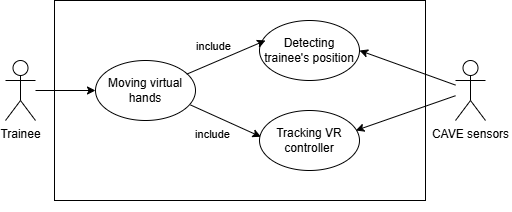
\includegraphics[width=0.7\textwidth]{Images/TraineeMovementUseCases.png}
	\caption{Use case diagram for trainee movement}
	\label{fig:movementDiagram}
\end{figure}
The use case descriptions for controlling trainee's movement are detailed in following subsections.

\subsubsection{Detecting trainee's position}
\begin{itemize}
\item Actors: Trainee, CAVE Sensors
\item Description: The system detects the change of the trainee's position.
\item Prerequisites: None.
\item Post-requisites: Data of the trainee's position is forwarded to the application's components.
\item Scenario: 
\begin{enumerate}
    \item The trainee moves inside CAVE.
    \item CAVE sensors read the trainee's movement data based on the VR controllers and glasses positions.
    \item The updated data is forwarded to the application's components.
\end{enumerate}

\end{itemize}
\subsubsection{Tracking VR controllers}
\begin{itemize}
\item Actors: Trainee, CAVE Sensors
\item Description: The system detects the change of the position or rotation of the VR controller.
\item Prerequisites: None.
\item Post-requisites: Data of the trainee's hand movement is forwarded to the application's components.
\item Scenario: 
\begin{enumerate}
    \item The trainee moves or rotates their hand.
    \item CAVE sensors read the updated position of VR controllers.
    \item The updated data is forwarded to the application's components.
\end{enumerate}
\end{itemize}

\subsubsection{Virtual hands movement}

\begin{itemize}
\item Actors: Trainee
\item Description: Virtual hands' position and rotation are updated according to trainee's movement.
\item Prerequisites: VR controllers movement or the trainee's position change were detected (Use cases: Detecting trainee's position, Tracking VR controllers).
\item Post-requisites: Virtual hands position parameters are updated.
\item Scenario: 
\begin{enumerate}
    \item The updated position and rotation vectors are read from the player control component.
    \item Virtual hands' position and rotation vectors are updated with the read values. 
\end{enumerate}

\end{itemize}

\subsection{Computer assembly use cases}
Figure \ref{fig:assemblyDiagram} illustrates the second use case diagram, describing the use cases for the computer assembly process, along with mechanics of trainee's score calculation and the computer work visualization.
\begin{figure}[H]
	\centering
		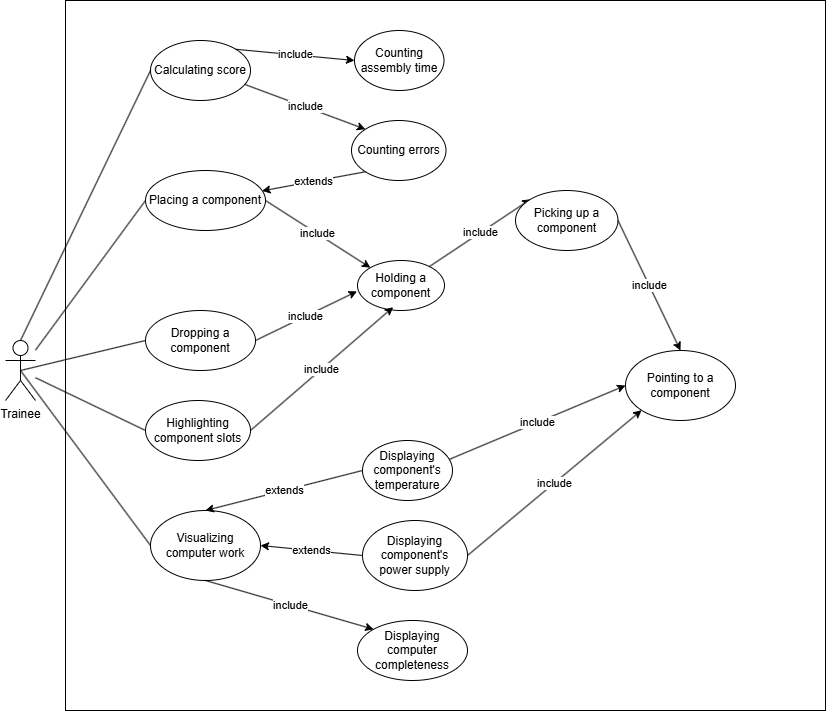
\includegraphics[width=0.7\textwidth]{Images/AssemblyUseCases.png}
	\caption{Use case diagram for computer assembly}
	\label{fig:assemblyDiagram}
\end{figure}

\noindent The following subsections provide the descriptions for the use cases.
\subsubsection{Detecting a holdable object}
\begin{itemize}
\item Actors: Trainee
\item Description: System detects the overlaps between a virtual hand and holdable objects.
\item Prerequisites: Virtual hand object is overlapping with one or more holdable objects.
\item Post-requisites: A holdable object becomes highlighted.
\item Scenario: 
\begin{enumerate}
    \item Trainee moves the virtual hand towards a holdable object.
    \item The system detects an overlap between a virtual hand and another object.
    \item A holdable object becomes highlighted using the virtual hand's color.
\end{enumerate}
\item Alternate scenario: The virtual hand object overlaps with multiple holdable objects at once.
\begin{enumerate}
    \item The system compares all of the objects overlapping with a virtual hand.
    \item The object with the smallest volume becomes selected and highlighted.
\end{enumerate}
\end{itemize}

\subsubsection{Picking up an object}
\begin{itemize}
\item Actors: Trainee
\item Description: Trainee picks up a holdable object.
\item Prerequisites: Holdable object overlaps with a virtual hand (Use case: Detecting a holdable object).
\item Post-requisites: A holdable object follows trainee's hand.
\item Scenario: 
\begin{enumerate}
    \item Trainee presses a trigger on the controller.
    \item System detects trainee's action.
    \item A holdable object begins following trainee's hand.
\end{enumerate}

\end{itemize}
\subsubsection{Holding an object}
\begin{itemize}
\item Actors: Trainee
\item Description: A held object's position and rotation follow the virtual hand.
\item Prerequisites: Trainee picks up a holdable object (Use case: Picking up an object).
\item Post-requisites: The held object continuously follows the virtual hand and updates its position and rotation.
\item Scenario: 
\begin{enumerate}
    \item The held object reads virtual hand object's position and rotation.
    \item The held object's position and rotation are updated with the obtained values.
\end{enumerate}
\end{itemize}

\subsubsection{Releasing an object}
\begin{itemize}
\item Actors: Trainee
\item Description: A holdable object becomes released and stops following trainee's virtual hand.
\item Prerequisites: Trainee holds an object (Use case: Holding an object).
\item Post-requisites: A held object either falls to the ground or becomes installed in the virtual computer (Use case: Installing a computer component).
\item Scenario: 
\begin{enumerate}
    \item Trainee presses a trigger on the controller.
    \item The released object stops being highlighted.
    \item The held object stops following trainee's hand.
    \item The released object falls to the ground.
\end{enumerate}
\item Alternate scenario: The released object is a computer component.
\begin{enumerate}
    \item The system checks whether the male slot of the released component overlaps with a female slot of another component.
    \item If the condition is met, the system attempts to install the released component in the slot it's overlapping with (Use case: Installing a computer component).
    \item Otherwise, the released component falls to the ground.
\end{enumerate}
\end{itemize}

\subsubsection{Installing a computer component}
\begin{itemize}
\item Actors: Trainee
\item Description: A computer component becomes intalled in the matching slot.
\item Prerequisites: Trainee releases the computer component while it overlaps with a component slot (Use case: Releasing an object).
\item Post-requisites: The computer component is either installed in the component slot or it falls to the ground.
\item Scenario: 
\begin{enumerate}
    \item Trainee releases the held object.
    \item System checks whether the component type matches the type of the slot it overlaps with.
    \item If the types match, the computer component's position becomes fixed and it snaps to the slot.
\end{enumerate}
\item Alternate scenario: The component is not compatible with the slot.
\begin{enumerate}
\item The released computer component falls to the ground.
\item The error counter increments (Use case: Counting trainee's errors).
\end{enumerate}
\end{itemize}


\subsubsection{Removing the computer component}
\begin{itemize}
\item Actors: Trainee
\item Decription: A computer component is removed from the slot.
\item Prerequisites: A computer component selected for removal is installed into one of the slots.
\item Post-requisites: Removed computer component falls down and can be picked up again.
\begin{enumerate}
    \item Trainee's virtual hand overlaps with an installed component (Use case: Detecting a holdable object).
    \item Trainee presses the button on a controller.
    \item System detects trainee's action.
    \item Removed component stops following the slot it was removed from.
\end{enumerate}


\end{itemize}

\subsubsection{Visualizing component's state}
\begin{itemize}
\item Actors: Trainee
\item Description: The parameters of a computer component is displayed to the trainee.
\item Prerequisites: Computer is fully built.
\item Post-requisites: Trainee sees component's state.
\item Scenario: 
\begin{enumerate}
    \item The trainee's virtual hand overlaps with a computer component installed in the virtual computer (Use case: Detecting a holdable object).
    \item System reads component's data.
    \item Read data is displayed to the trainee using an application's interface.
\end{enumerate}

\end{itemize}

\subsubsection{Displaying assembly progress}
\begin{itemize}
\item Actors: Trainee
\item Description: The system informs the trainee about the progress of the virtual computer assembly as a list of objectives.
\item Prerequisites: The trainee installs a computer component (Use case: Installing a computer component).
\item Post-requisites: The system updates and displays the list of objectives according to the virtual computer assembly progress.
\item Scenario: 
\begin{enumerate}
    \item The system checks which components are installed in the virtual computer.
    \item The system updates the list of objectives accordingly to the progress of the virtual computer assembly.
    \item The system displays the updated list of objectives in an application's interface.
\end{enumerate}
\end{itemize}

\subsubsection{Visualizing computer work}
\begin{itemize}
\item Actors: Trainee
\item Description: The system displays information about the virtual computer assembly progress or a state of the computer components to the trainee.
\item Prerequisites: None.
\item Post-requisites: The system presents necessary information using an application's interface.
\item Scenario: 
\begin{enumerate}
    \item The system validates the state of the virtual computer.
    \item If the virtual computer is not fully assembled, the system displays information about the progress of the assembly process (Use case: Displaying assembly progress).
\end{enumerate}
Alternate scenario: The virtual computer is fully assembled and the virtual hand object is overlapping with one of its components (Use case: Detecting a holdable object).
\begin{enumerate}
    \item The system displays information about the component's state to the trainee (Use case: Visualizing component's state).
\end{enumerate}
\end{itemize}


\subsubsection{Counting assembly time}  
\begin{itemize}
\item Actors: Trainee
\item Description: Time of the assembly is presented to the trainee.
\item Prerequisites: Trainee picks up a computer component for the first time (Use case: Picking up an object).
\item Post-requisites: Time becomes displayed in the application's interface.
\item Scenario: 
\begin{enumerate}
    \item System checks if the computer assembly process is not finished.
    \item System calculates the elapsed assembly time.
    \item The time value becomes displayed in the application's interface clock object.
\end{enumerate}
Alternate scenario: The computer assembly is finished.
\begin{enumerate}
    \item The clock object stops updating the time.
\end{enumerate}
\end{itemize}

\subsubsection{Counting trainee's errors}
\begin{itemize}
\item Actors: Trainee
\item Description: The system counts the trainee's mistakes during the virtual computer assembly process.
\item Prerequisites: Trainee installs a computer component in an incompatible slot (Use case: Installing a computer component). 
\item Post-requisites: Error counter is updated and displayed in the application's interface.
\item Scenario: 
\begin{enumerate}
    \item System increments the error counter.
    \item The updated error count becomes displayed in the application's interface.
\end{enumerate}

\end{itemize}

\subsubsection{Tracking trainee's score}
\begin{itemize}
\item Actors: Trainee
\item Description: Trainee's score is calculated based on the time and quality of a computer assembly process.
\item Prerequisites: The virtual computer is fully assembled.
\item Post-requisites: The trainee's score is displayed in an application's interface.
\item Scenario: 
\begin{enumerate}
    \item The trainee's score is initialized with a constant value.
    \item The system decreases the score by a constant value for each 10 seconds of the assembly process (Use case: Counting assembly time).
    \item The system decreases the score by a constant value for each mistake made by the trainee (Use case: Counting trainee's errors).
    \item System displays score in the application's interface.
\end{enumerate}

\end{itemize}
% popraw
\section{Classes}
\label{sec:classes}
A class is a fundamental element of OOP (Object-Oriented Programming).
It's a definition describing an object's state or behaviour using certain attributes or methods. 
The following subsections presents the developed classes along with the class diagram.
\subsection{Class diagram}
A class diagram is an essential element of a system project.
It allows to visualize the project's structure as well as relationships and dependencies of the classes.
Figure \ref{fig:movementDiagram} provides a full class diagram for the project.
\begin{figure}[H]
	\centering
		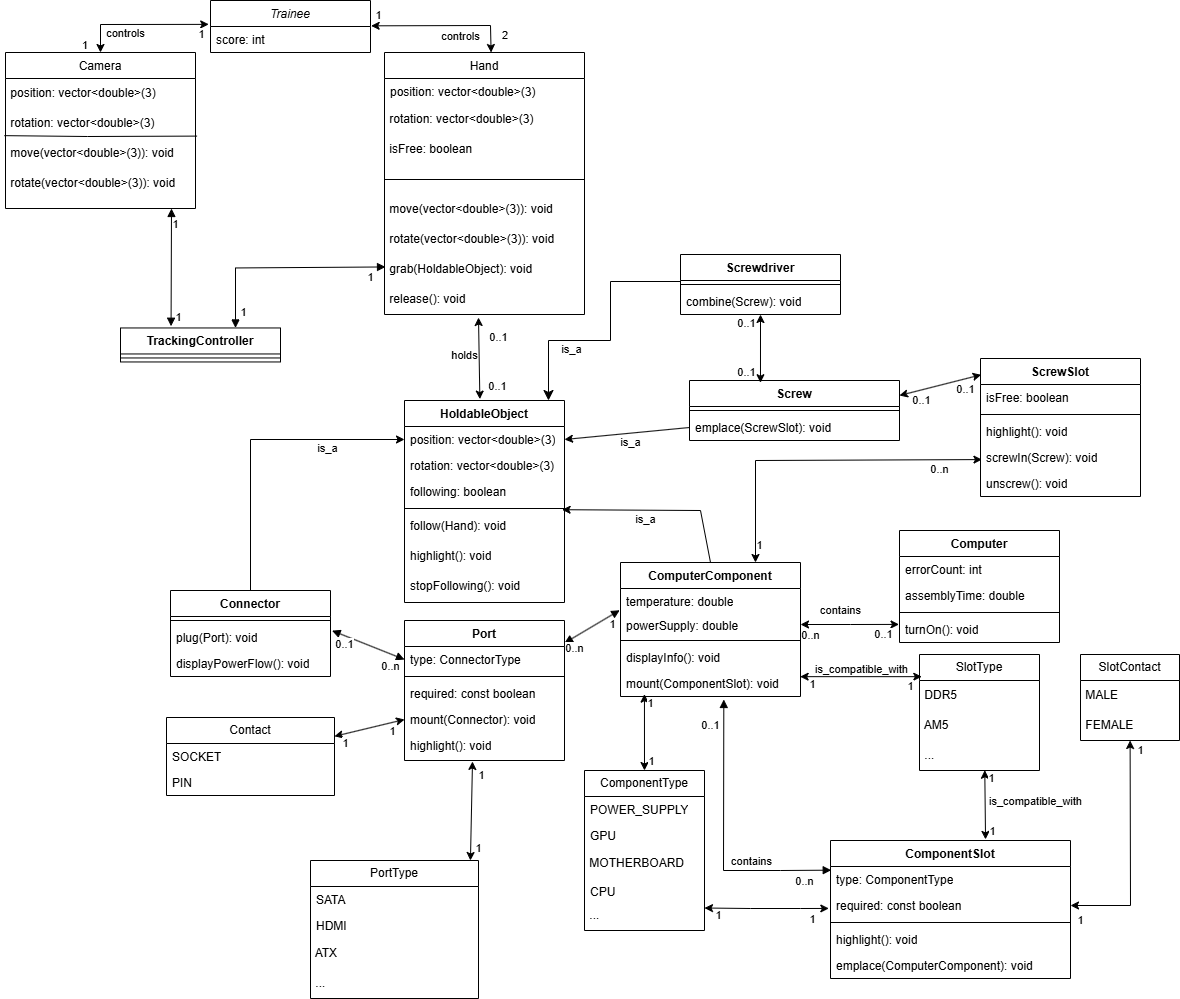
\includegraphics[width=0.7\textwidth]{Images/Class_diagram.png}
	\caption{Class diagram}
	\label{fig:ClassDiagram}
\end{figure}
The trainee-related classes (figure \ref{fig:TraineeClasses}) are responsible of detecting trainee's movement and calculating their score.
A Camera class describes the behavior of a virtual camera object, which acts as a trainee's point of view in a VR environment.
The Hand class is responsible for moving the virtual hands objects.
Both of the described classes are using the TrackingController class, which is responsible for detecting the movement of a trainee in the VR CAVE and forwarding its data to these classes.
\begin{figure}[H]
	\centering
		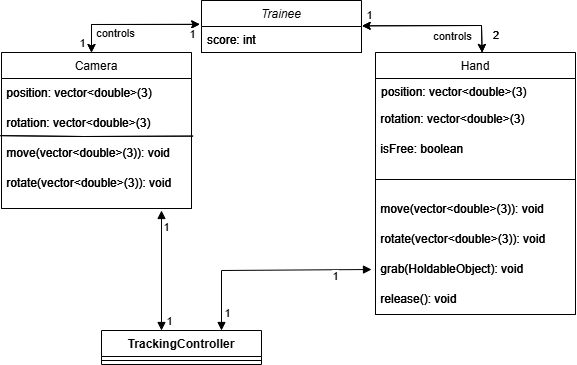
\includegraphics[width=0.7\textwidth]{Images/TraineeRelatedClasses.png}
	\caption{Trainee-related classes}
	\label{fig:TraineeClasses}
\end{figure}
A HoldableComponent class (figure \ref{fig:HoldableComponentClasses}) describes each object, which can be manipulated by trainee by holding it and moving it around.
These classes are elements or tools required to build a virtual computer.
If the trainee grabs one of these objects and moves, the held object should follow their hands' position.
Releasing the held object makes it fall to the ground and return to its initial position.

\begin{figure}[H]
	\centering
		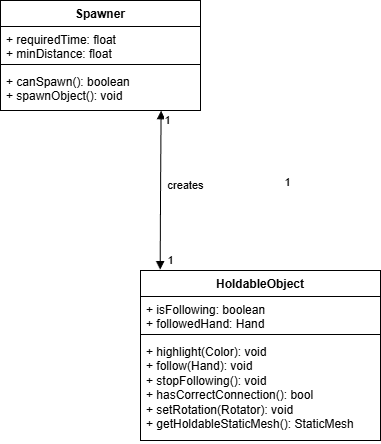
\includegraphics[width=0.7\textwidth]{Images/HoldableComponentClasses.png}
	\caption{Holdable Components classes}
	\label{fig:HoldableComponentClasses}
\end{figure}

A Connector class (figure \ref{fig:ConnectorRelatedClasses}) describes objects, which connect two or more computer components with eahc other.
Each connector has one or more ports.
Every port is described by a type and a contact, which are stored in PortType and Contact enumeration classes.
To properly mount a connector, all of his ports have to be connected with a port of the same type and an opposite contact. 
The power flow of the connectors may also be visualized after turning on a fully built computer. 
\begin{figure}[H]
	\centering
		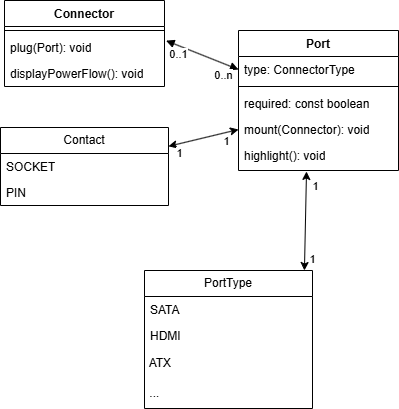
\includegraphics[width=0.7\textwidth]{Images/ConnectorRelatedClasses.png}
	\caption{Connector-related classes}
	\label{fig:ConnectorRelatedClasses}
\end{figure}
Figure \ref{fig:ToolsRelatedClasses} presents the Screwdriver and Screw classes, which describe the objects for tools used during the virtual computer assembly.
A held screwdriver object can be connected with a screw by contacting them with each other.
A screw can be emplaced in a ScrewSlot object, when a trainee holds the connected screwdriver and screw objects, moves their hand near the slot and rotates it.

\begin{figure}[H]
	\centering
		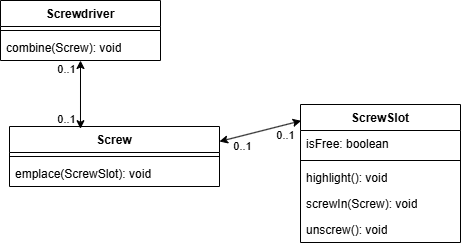
\includegraphics[width=0.7\textwidth]{Images/ToolsRelatedClasses.png}
	\caption{Tools-related classes}
	\label{fig:ToolsRelatedClasses}
\end{figure}


A virtual computer (figure \ref{fig:ComputerRelatedClasses}) consists of multiple computer components.
Each computer component object can be mounted in a ComponentSlot object.
To mount a component in a slot, the types of the component and the slot, which are listed in ComponentType and PortType enumerations, must be equal.
Some components may contain connector ports and slots for the screws or another components.
Most of the components have parameters which values may be continously changing and visualized after turning on a fully built computer.

\begin{figure}[H]
	\centering
		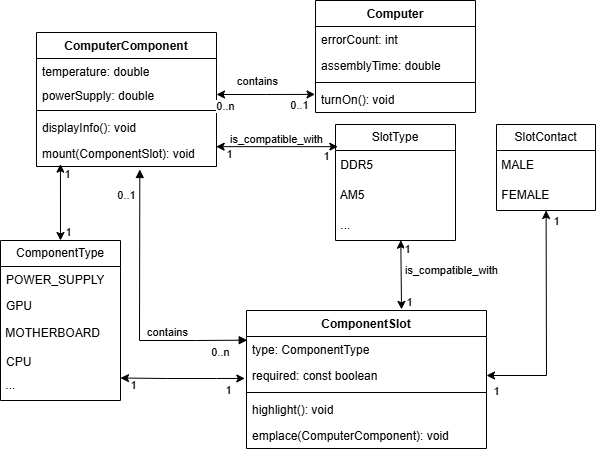
\includegraphics[width=0.7\textwidth]{Images/ComputerRelatedClasses.png}
	\caption{Computer-related classes}
	\label{fig:ComputerRelatedClasses}
\end{figure}